\section{Derivative}

The gravitational potential generated by the Earth in space, at a point at a
distance $r$ from its center, is given by:
\[
U(r) = -\frac{GM}{r}
\]
where $M$ is the mass of the Earth and $G$ is the universal gravitational
constant. The function $U(r)$ is not at all linear. However, if we consider the
gravitational field for points near the Earth's surface, we expect an
approximately linear behavior. Let us try to make this idea explicit.

Suppose we are at a height $h$ from the Earth's surface. We will then be at a
distance $R+h$ from the center of the Earth. Thus, we have:
\[
  U(R+h) = -GM\frac{1}{R+h}.
\]
Now observe that
\begin{align*}
  \frac{1}{R+h}
  & = \frac{1}{R} + \frac{1}{R+h} - \frac{1}{R}
   = \frac 1 R + \frac{R-(R+h)}{R(R+h)} \\
  & = \frac 1 R - \frac{h}{R(R+h)} \\
  & = \frac 1 R - \frac{h}{R^2} - \frac{h}{R(R+h)} + \frac{h}{R^2} \\
  & = \frac 1 R - \frac{h}{R^2} - \frac{hR - h(R + h)}{R^2(R+h)} \\
  & = - \frac{h}{R^2} + \frac 1 R + \frac{h^2}{R^2(R+h)}.
\end{align*}
Thus, we have
\begin{align*}
  U(R+h) &= \frac{GM}{R^2} h - \frac{GM}{R} + \omega(h)\\
  &= g h + C + \omega(h)
\end{align*}
where $g = GM/R^2$, $C$ is a constant (irrelevant because the potential can be
defined up to a constant), and $\omega(h)$ is a function with the property
$\omega(h)/h\to 0$ as $h\to 0$. Thus, if $h$ is very small compared to $R$, the
term $\omega(h)$ is negligible compared to the term $gh$ (even though both tend
to zero as $h\to 0$). This justifies the use of the simplified formula:
\[
U_0(h) = gh
\]
from which the potential energy $E = mgh$ is derived if we have a mass $m$ at a
height $h$ on the Earth's surface.

\begin{figure}
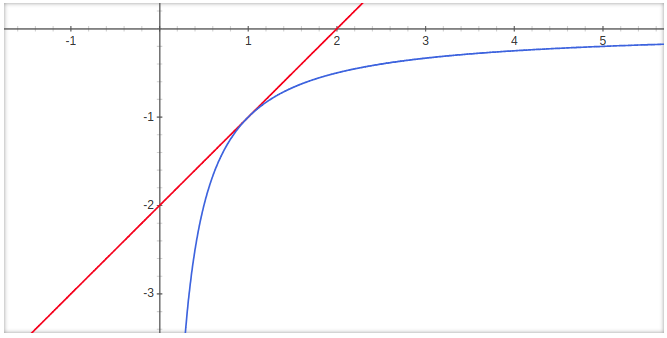
\includegraphics[width=0.49\textwidth]{derivata_00.png}\hfill%
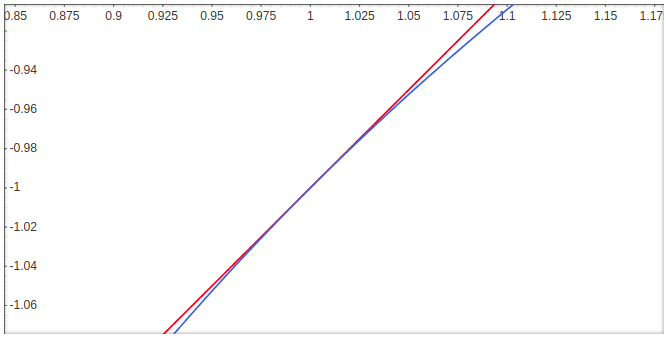
\includegraphics[width=0.49\textwidth]{derivata_01.png}
\label{fig:derivata}
\caption{The graph of the Earth's gravitational potential.
On the $x$-axis, the distance from the Earth's center in Earth radii.
On the $y$-axis, the gravitational potential with units $C=GM/R$.
The slope of the tangent line to the graph of the curve at $x=R$ is $g=GM/R^2$.
In the right figure, an enlargement around the Earth's radius: it is noted how
the graph of the potential is almost indistinguishable from the graph of the
tangent line.}
\end{figure}

What we have done is a process of \emph{linearization}%
\mymargin{linearization}%
\index{linearization}. 
The gravitational field is described by a nonlinear function: $-GM/r$.
But when we restrict to a small interval of values of $r$ 
(the values of $r$ close to $R$, the Earth's radius), such a function 
is almost indistinguishable, up to a constant, from the linear function 
$gh$ if $r=R+h$.
Linear functions are much simpler to handle, and it is therefore convenient, 
if we remain on the Earth's surface, to use this latter formula for 
the gravitational potential.
The graph of the linear function that best approximates the graph of a 
function is called the \emph{tangent line}%
\mymargin{tangent line}%
\index{tangent line}. 
Its slope, $g$ in our example, is called the \emph{derivative}%
\mymargin{derivative}%
\index{derivative}.

Once derivatives are introduced, we will see that what we have
determined is the formula:
\[
U(R+h) = U(R) + U'(R) h + \omega(h).
\]

\begin{definition}[derivative]
\mymark{***}%
Let $A\subset \RR$, $f\colon A \to \RR$, 
$x_0\in A$ be an accumulation point of $A$.
We will say that the function $f$ is \emph{differentiable} at the point $x_0$ if
the following limit exists and is finite:
\[
  \lim_{h\to 0} \frac{f(x_0+h) - f(x_0)}{h}.
\]
In such a case, we will denote by $f'(x_0)$ the value of this limit, which we
will call the \emph{derivative}%
\mymargin{derivative}%
\index{derivative} of the function $f$ at the point $x_0$.

If $B$ is the set of accumulation points of $A$ where $f$ is differentiable,
then the derivative function $f'\colon B \to \RR$ is defined.

A function $f$ is said to be differentiable if it is differentiable at every
point of its domain.
If $C\subset A$, the function $f$ is said to be \emph{differentiable on $C$} if
it is differentiable at every point of the set $C$ (i.e., if $C\subset B$).

Alternative notations for denoting the derivative of a function:
\[
  f' = Df = \frac{d}{dx} f = \frac{df}{dx}.
\]

The definition of derivative extends formally identically 
to functions of a complex variable and/or with complex values.
The derivative of a function with complex values is
itself with complex values.
\end{definition}

The ratio
\[
\frac{f(x_0+h) - f(x_0)}{h}
\]
is called the \emph{incremental ratio}%
\mymargin{incremental ratio}%
\index{incremental ratio}. In fact, by changing the variable and setting $x=x_0+h$, it can be written as
\[
\frac{f(x_0+h) - f(x_0)}{h}
= \frac{f(x) - f(x_0)}{x-x_0}
= \frac{\Delta f}{\Delta x}
\]
which turns out to be the ratio of the increment of the function $f$ (sometimes
denoted by $\Delta f$) with respect to the corresponding increment of the
variable $x$ (sometimes denoted by $\Delta x$).
By changing the variable in the limit, as $h\to 0$, we have $x\to x_0$
and thus
\[
 f'(x_0) = \lim_{x\to x_0} \frac{f(x)-f(x_0)}{x-x_0}.
\]

If $f$ is differentiable at the point $x_0$,
the line with equation 
\mymargin{tangent line}%
\begin{equation}\label{eq:retta_tangente}
  y = f(x_0) + f'(x_0) \cdot (x-x_0)  
\end{equation}
is the unique line passing through the point $(x_0,f(x_0))$ 
with a slope equal to the derivative $f'(x_0)$.
This line is called the \emph{tangent line}
\index{tangent line}%
\index{tangent!to the graph}%
to the graph of the function $f$ at the point $(x_0,f(x_0))$.
It is the line that best approximates the graph of $f$ 
as $x\to x_0$ in the sense that it results in:
\[
  \lim_{x\to x_0} \frac{f(x) - [f(x_0)+f'(x_0)(x-x_0)]}{x-x_0} = 0
\]
while any other line would make this limit infinite.

\begin{example}%
\label{ex:derivata_reciproco}%
\mymark{**}%
Consider the function $f(x) = 1/x$ defined on the set $A = \RR \setminus
\ENCLOSE{0}$. Then for every $x\neq 0$:
\[
  f'(x) = \lim_{h\to 0} \frac{\frac{1}{x+h} - \frac{1}{x}}{h}
        = \lim_{h\to 0} \frac{x - (x+h)}{h(x+h)x}
        = \lim_{h\to 0} \frac{-1}{(x+h)x} = -\frac{1}{x^2}.
\]
Thus, the function $1/x$ is differentiable, and its derivative is the function
$-1/x^2$.
\end{example}

\begin{theorem}[continuity of differentiable functions]
\mymark{***}
If $f$ is differentiable at the point $x$, then $f$ is also continuous at the
point $x$.
\end{theorem}
%
\begin{proof}
\mymark{***}
We have
\[
  \lim_{h\to 0} f(x+h) - f(x) = \lim_{h\to 0} \frac{f(x+h) - f(x)}{h} \cdot h
  = f'(x) \cdot 0 = 0.
\]
Thus, $f(x+h)\to f(x)$ as $h\to 0$, and therefore $f$ is continuous at the point
$x$.
\end{proof}

\begin{example}[continuous but not differentiable function]
\mymark{***}
The function $f(x) = \abs{x}$ is an example of a continuous but not
differentiable function. It is indeed easy to verify that at the point $x_0=0$,
the
right-hand limit of the incremental ratio is $1$, while the left-hand limit is
$-1$.

Another example is the function $f(x) = \sqrt{x}$, which is continuous but not
differentiable at the point $x_0=0$ because the limit of the incremental ratio
exists but is $+\infty$.
\end{example}

\begin{theorem}[derivative of the composite function]
\mymark{**}%
Let $f$ be a function differentiable at the point $x_0$
and let $g$ be a function differentiable at the point $f(x_0)$.
Then the composite function $g\circ f$ is differentiable
at the point $x_0$, and we have:
\[
  (g\circ f)'(x_0) = g'(f(x_0))\cdot f'(x_0).
\]
\end{theorem}
%
\begin{proof}
\mymark{**}
Consider the function
\[
  G(y) =
  \begin{cases}
   \frac{g(y) - g(f(x_0))}{y-f(x_0)} & \text{if $y \neq f(x_0)$},\\
   g'(f(x_0)) & \text{if $y=f(x_0)$}.
  \end{cases}
\]
Then we have
\begin{equation}\label{eq:47439}
 \frac{g(f(x_0+h))-g(f(x_0))}{h}
 = G(f(x_0+h)) \cdot \frac{f(x_0+h)-f(x_0)}{h}
\end{equation}
indeed, if $f(x_0+h)\neq f(x_0)$, we have multiplied and divided
by $f(x_0+h) - f(x_0)$; if instead $f(x_0+h)=f(x_0)$, then also
$g(f(x_0+h))=g(f(x_0))$, and the equality is still valid because both the
left-hand side and the right-hand side are zero (and the value assigned to $G$
is irrelevant in this case).

Clearly, as $h\to 0$, the second factor on the right-hand side
of the equality \eqref{eq:47439}
tends, by definition, to $f'(x_0)$.
Regarding the first factor,
we observe that $G(y)$, as defined, is a continuous function at the point
$y=f(x_0)$ because
\[
\frac{g(y) - g(f(x_0))}{y-f(x_0)} \to g'(f(x_0))
\]
as $y\to f(x_0)$.
But also the function $f$ is continuous at the point $x_0$ (since it is
differentiable by hypothesis).
Thus, the composite function $G(f(x_0+h))$ is continuous at the point $h=0$.
Therefore, $G(f(x_0+h)) \to G(f(x_0)) = g'(f(x_0))$ as $h\to 0$.
Thus, the right-hand side of \eqref{eq:47439} has the limit $g'(f(x_0)) \cdot
f'(x_0)$ as $h\to 0$, as we wanted to demonstrate.
\end{proof}

\begin{theorem}[derivative of the inverse function]
\mymark{**}
Let $f$ be an invertible function differentiable at a point $x_0$ and
suppose that the inverse function $f^{-1}$ is continuous at $f(x_0)$.
If $f'(x_0)\neq 0$, then $f^{-1}$ is differentiable at $f(x_0)$, and we have:
\[
  (f^{-1})'(f(x_0)) = \frac{1}{f'(x_0)}.
\]
Letting $y_0 = f(x_0)$, the formula can also be written in the form:
\[
  (f^{-1})'(y_0) = \frac{1}{f'(f^{-1}(y_0))}.
\]
If instead $f'(x_0)=0$, the function $f^{-1}$ is not differentiable at $f(x_0)$.
\end{theorem}
%
Observe that 
if $I$ is an interval,
and if $f\colon I\to \RR$,
is injective and continuous, then $J=f(I)$ is an interval
and the inverse function $f^{-1}\colon J\to I$
is continuous (Exercise~\ref{ex:inversa_monotona}).
%
\begin{proof}
\mymark{**}
Let $y_0 = f(x_0)$ and consider the incremental ratio of $f^{-1}$ at the point
$y_0$:
\[
  \frac{f^{-1}(y) - f^{-1}(y_0)}{y-y_0}.
\]
As $y\to y_0$, we can change the variable
$x=f^{-1}(y)$ since we have assumed that $f^{-1}$ is continuous at $f(x_0)$, so
we know that as $y\to y_0$, $x = f^{-1}(y)\to f^{-1}(y_0) = x_0$.
Thus, as $y\to y_0$, $x\to x_0$, and,
if $f'(x_0)\neq 0$:
\[
  \frac{f^{-1}(y) - f^{-1}(y_0)}{y-y_0}
  = \frac{x-x_0}{f(x)-f(x_0)}
  = \frac{1}{\frac{f(x)-f(x_0)}{x-x_0}} \to \frac{1}{f'(x_0)}.
\]

If instead $f'(x_0)=0$, the incremental ratio of the inverse function
has an infinite limit, and therefore the inverse function is not differentiable
at $f(x_0)$.
\end{proof}

\begin{theorem}[operations with derivatives]
  \label{th:derivate_operazioni}%
\mymark{***}%
Let $f$ and $g$ be two functions differentiable at the same point $x_0$.
Then the functions $f+g$, $f-g$, $f\cdot g$, and, if $g(x_0)\neq 0$, also $f/g$
are differentiable at $x_0$. At points where both functions are differentiable,
we have
\begin{gather*}
  (f+g)' = f' + g', \qquad
  (f-g)' = f' - g', \\
  (f\cdot g)' = f' \cdot g + f g', \qquad
  \enclose{\frac{f}{g}}' = \frac{f'g - fg'}{g^2}.
\end{gather*}
\end{theorem}
%
\begin{proof}
\mymark{***}
Regarding the derivative of the sum (or difference), it is sufficient to observe
that the incremental ratio of the sum (or difference) is the sum (or difference)
of the incremental ratios and that the limit of the sum (or difference) is equal
to the sum (or difference) of the limits.

We calculate the derivative of the product $f\cdot g$ at the point $x_0$. We
have
\begin{align*}
  \frac{f(x)g(x) - f(x_0)g(x_0)}{x-x_0}
  &= \frac{f(x)(g(x) - g(x_0)) + (f(x)-f(x_0))g(x_0)}{x-x_0}\\
  &= f(x) \frac{g(x)-g(x_0)}{x-x_0} + \frac{f(x)-f(x_0)}{x-x_0} g(x_0).
\end{align*}
Passing to the limit as $x\to x_0$, we remember that $f(x)\to f(x_0)$ since $f$
is continuous at $x_0$ (being differentiable by hypothesis). The incremental
ratios tend to the derivatives, and we obtain the desired result $f(x_0) g'(x_0)
+ f'(x_0) g(x_0)$.

Regarding the derivative of the quotient, we observe that
letting $h(y)=1/y$, we have
\[
  \frac{f(x)}{g(x)} = f(x) \cdot h(g(x)).
\]
From example~\ref{ex:derivata_reciproco}, we know that $h'(y) = -1/y^2$, and
thus
we can use the formulas for the derivative of the product and the derivative of
the composite function to obtain:
\begin{align*}
  \enclose{\frac{f}{g}}'(x_0)
  &= \enclose{f \cdot (g\circ h)}'(x_0) \\
  &= f'(x_0) \cdot h(g(x_0)) + f(x_0) \cdot h'(g(x_0))\cdot g'(x_0)\\
  &= \frac{f'(x_0)}{g(x_0)} + f(x_0) \cdot \frac{-1}{g^2(x_0)} g'(x_0)\\
  &= \frac{f'(x_0)g(x_0) - f(x_0)g'(x_0)}{g^2(x_0)}.
\end{align*}
\end{proof}

\begin{table}
  \begin{tabular}{c|c||c|c||c|c}
    $f(x)$ & $f'(x)$ & $f(x)$ & $f'(x)$ & $f(x)$ & $f'(x)$
    \\\hline
    $mx + q$ & $m$ &
    $e^x$ & $e^x$ &
    $\sin x$ & $\cos x$ \\
    $\abs{x}$ & $\frac{x}{\abs{x}}$ &
    $\ln x$ & $\frac 1 x$ &
    $\cos x$ & $-\sin x$ \\
    $x^n$ & $n x^{n-1}$ &
    $\sinh x$ & $\cosh x$ &
    $\arcsin x$ & $\frac{1}{\sqrt{1-x^2}}$ \\
    $x^\alpha$ & $\alpha x^{\alpha -1}$ &
    $\cosh x$ & $\sinh x$ & $\arccos x$ & $-\frac{1}{\sqrt{1-x^2}}$ \\
    $\sqrt[n]{x}$ & $\frac{1}{n\sqrt[n]{x^{n-1}}}$ &
    $\settsinh x$ & $\frac{1}{\sqrt{x^2+1}}$ &
    $\tg x$ & $1+ \tg^2 x$ \\
    $\sqrt{x}$ & $\frac{1}{2\sqrt{x}}$ &
    $\settcosh x$ & $\frac{1}{\sqrt{x^2-1}}$ &
    $\arctg x$ & $\frac{1}{1+x^2}$
  \end{tabular}
  \caption{Derivatives of elementary functions}
  \label{tab:derivate}%
\end{table}

\begin{theorem}[derivatives of elementary functions]%
\label{th:derivate_elementari}%
\index{derivative!of elementary functions}%
\mymark{**}%
For $m,q,\alpha \in \RR$, $\alpha \neq 0$, $n\in \NN$, $n\neq 0$,
the differentiation rules summarized in
table~\ref{tab:derivate} hold: the functions in the column
$f(x)$ have the derivative reported in the column $f'(x)$.
The functions $f(x)$ are differentiable at the points of their domain 
where the corresponding expression $f'(x)$ is well-defined.
In particular:
the function $\sqrt[n]{x}$
is not differentiable at $x=0$,
the functions $\arcsin x$ and $\arccos x$ are not differentiable at the points
$-1$ and $1$,
the function $\abs{x}$ is not differentiable at $0$,
the function $\settcosh x$ is not differentiable at $1$,
the function $\ln x$ is differentiable for every $x>0$.
Linear functions, powers with positive base, powers with integer exponent,
exponential, logarithm, sine, cosine, tangent, arctangent are instead
differentiable
at all points where they are defined.
\end{theorem}

\begin{proof}
\mymark{**}
For linear functions, we have:
\begin{align*}
(mx+q)' &= \lim_{h\to 0}\frac{m(x+h)+q - (mx+q)}{h} = \lim_{h\to 0} m = m.
\end{align*}
Recalling that the derivative is a limit and that the limit at a point depends 
only on the values of the function in a neighborhood of the point, 
we can assert that the derivative of the absolute value $\abs{x}$ 
coincides with the derivative of $x$, i.e., $1$ for $x>0$, and coincides 
with the derivative of $-x$ for $x<0$. Thus, $D \abs{x} = x / \abs{x}$ 
if $x\neq 0$. 
If $x=0$, the right and left limits of the incremental ratio of $\abs{x}$ 
tend to $1$ and $-1$, respectively, and therefore the derivative does not exist.

We prove that $Dx^n = n x^{n-1}$ for $n\in \NN$, $n>0$, 
by induction on $n$. For $n=1$, we have $x^n=x^1$, which is linear, 
and thus from the previous formula, $Dx^1 = 1 = 1 \cdot x^0$. 
Assuming we know that $D x^n = n x^{n-1}$, we have, applying 
the product differentiation rule:
\[
  D x^{n+1} = D x\cdot x^n = 1 \cdot x^n + x \cdot n x^{n-1}
   = x^n + n x^n = (n+1) x^n
\]
thus proving the inductive step.
Recalling the formula for the derivative of the quotient,
we can find the formula for powers with negative integer exponent:
\[
  D x^{-n} = D \frac{1}{x^n} = \frac{-n x^{n-1}}{x^{2n}}
   = -n x^{n-1-2n} = -n x^{-n-1}.
\]

The derivative of the $n$-th root is found using the formula for the derivative
of the inverse function $x^n$, which can be applied if $x\neq 0$:
\[
  D \sqrt[n]{x} = \frac{1}{n(\sqrt[n]{x})^{n-1}}
    = \frac{1}{n\sqrt[n]{x^{n-1}}}.
\]
Note that if $n$ is odd, the formula is valid even for $x<0$.
The derivative of the square root is obtained by setting $n=2$.

Regarding the derivative of the exponential,
we relate it to a notable limit:
\[
  D e^x = \lim_{h\to 0} \frac{e^{x+h}-e^x}{h}
  = \lim_{h\to 0}\frac{e^x e^h - e^x}{h}
  = \lim_{h\to 0}e^x \frac{e^h - 1}{h}
  = e^x.
\]
The derivative of the logarithm is obtained as the derivative of the inverse
function of the exponential:
\[
  D \ln x = \frac{1}{e^{\ln x}} = \frac{1}{x} \qquad\text{for $x>0$}.
\]
We can then calculate the derivative of powers with positive base and any real
exponent:
\[
D x^\alpha
= D e^{\alpha \ln x}
= e^{\alpha \ln x} D(\alpha \ln x)
= x^\alpha \alpha \frac{1}{x}
= \alpha x^{\alpha -1}.
\]

Regarding the trigonometric functions 
$\sin$ and $\cos$, we recall the notable limit
(theorem~\ref{th:limite_notevole_sin})
\[
  \lim_{h\to 0}\frac{\sin h}{h} = 1
\]
from which we derive, as $h\to 0$, 
\[
\frac{1-\cos h}{h}
= \frac{1-\cos^2 h}{h\cdot(1+\cos h)}
= \frac{\sin^2 h}{h\cdot (1+\cos h)}
= \frac{\sin h}{h} \cdot \frac{\sin h}{1+\cos h}
\to 1 \cdot \frac{0}{2} = 0.
\]
Applying the addition formulas, we have
\begin{align*}
  D \sin x
  &= \lim_{h\to 0}\frac{\sin(x+h)-\sin(x)}{h} \\
  &= \lim_{h\to 0}\frac{\sin(x)\cos(h) + \cos(x)\sin(h) - \sin(x)}{h} \\
    &= \lim_{h\to 0}\Enclose{\sin(x) \frac{\cos h-1}{h} + \cos(x) \frac{\sin
  h}{h}}
  = \cos(x).
\end{align*}
and similarly
\begin{align*}
  D \cos x
  &= \lim_{h\to 0}\frac{\cos(x+h)-\cos(x)}{h} \\
  &= \lim_{h\to 0}\frac{\cos(x)\cos(h) - \sin(x)\sin(h) - \cos(x)}{h} \\
    &= \lim_{h\to 0}\cos(x) \frac{\cos h-1}{h} - \sin(x) \frac{\sin h}{h} =
  -\sin(x)
\end{align*}

The function $\arcsin$ is defined as the inverse of the restriction of the
function $\sin$ to the interval $[-\pi/2, \pi/2]$.
In the open interval $(-\pi/2,$ $\pi/2)$, the function $\sin$ has a positive
derivative, and thus it follows that the inverse function (which we know to be
continuous) is differentiable in $(-1,1)$, and its derivative is
\[
D\arcsin x
= \frac{1}{\cos(\arcsin x)}
= \frac{1}{\sqrt{1-\sin^2 \arcsin x}}
= \frac{1}{\sqrt{1-x^2}}.
\]
Indeed, $\cos y = \sqrt{1-\sin^2 y}$ if $y\in [-\pi/2, \pi/2]$.

Similarly, the function $\arccos$ is defined as the inverse of the restriction
of $\cos$ to the interval $[0,\pi]$, and thus, for $x\in (-1,1)$,
\[
D \arccos x
 = \frac{1}{-\sin(\arccos x)}
 = \frac{1}{-\sqrt{1-\cos^2 \arccos x}}
 = -\frac{1}{\sqrt{1-x^2}}.
\]
Indeed, $\sin y = \sqrt{1-\cos^2 y}$ if $y\in[0,\pi]$.

At the points $x=1$ and $x=-1$, the functions $\arcsin$ and $\arccos$ are not
differentiable.

For the tangent function, we can use the formula for the derivative of the
quotient:
\begin{align*}
  D \tg x &= D \frac{\sin x }{\cos x}
   = \frac{\cos x \cdot \cos x - \sin x \cdot (-\sin x)}{\cos^2 x} \\
   &= \frac{\cos^2 x + \sin^2 x}{\cos^2 x}
   = 1 + \tg^2 x = \frac{1}{\cos^2 x}.
\end{align*}
Using the formula for the derivative of the inverse function, we have
\[
  D \arctg x = \frac{1}{1+\tg^2(\arctg x)}
  = \frac{1}{1+x^2}.
\]

Regarding the hyperbolic functions, the derivatives of $\sinh$
and $\cosh$ are immediately related to the derivative of the exponential,
using
definition~\eqref{eq:sinh_cosh}. The derivatives of the inverse functions
$\settsinh$ and $\settcosh$ are obtained from the formula for the derivative
of the inverse function and using
the relations $\cosh x = \sqrt{\sinh^2 x+1}$ and, for $x > 0$,
$\sinh x = \sqrt{\cosh^2 x -1}$:
\begin{align*}
  D \settsinh x &= \frac{1}{\cosh(\settsinh x)}
  = \frac{1}{\sqrt{\sinh^2 (\settsinh x) + 1}} = \frac{1}{\sqrt{x^2+1}}\\
  D \settcosh x &= \frac{1}{\sinh(\settcosh x)}
  = \frac{1}{\sqrt{\cosh^2(\settcosh x)-1}}
  = \frac{1}{\sqrt{x^2-1}}
\end{align*}
\end{proof}

Note that the differentiation rules just demonstrated 
are also valid for the complex functions $z^n$ and $e^z$:
in particular, $D z^n = nz^{n-1}$ for every $n\in \ZZ$,
$n\neq 0$, and $D e^z = e^z$ since the notable 
limit of the exponential is valid even in the complex field.
Other functions such as $\sqrt{x}$ 
or $\ln x$ are not uniquely extendable over $\CC$
and therefore require a separate theory. 
Once defined, however, it could be verified 
that these functions also satisfy the same differentiation rules 
as their real restrictions.

\begin{proposition}[Feynman's trick for derivatives]
  \index{Feynman's trick}%
  \index{Feynman's trick!for derivatives}%
  \index{Feynman!trick for derivatives}%
Let $f_1,\dots, f_n$ be differentiable functions and let $\alpha_1,\dots,
\alpha_n$
be real exponents. Then:
  \[
  \enclose{\prod_{k=1}^n f_k^{\alpha_k}}'
  = \prod_{k=1}^n f_k^{\alpha_k} \cdot \sum_{k=1}^n \alpha_k \frac{f_k'}{f_k}.
  \]
\end{proposition}
\begin{proof}
It suffices to observe that 
\begin{align*}
  \enclose{\prod_{k=1}^n f_k^{\alpha_k}}'
  &= \sum_{k=1}^n \alpha_k f_k' f_k^{\alpha_k-1} \prod_{j\neq k} f_j^{\alpha_j}
  = \sum_{k=1}^n \alpha_k \frac{f_k'}{f_k} \prod_{j=1}^n f_j^{\alpha_j}.
\end{align*}
\end{proof}
For example, if we want to calculate the derivative of the function 
\[
 f(x) = \frac{\sqrt{1-x^2}\cdot \ln x}{x\cdot \cos^2 x}
 = (1-x^2)^{\frac 1 2} \cdot \ln x \cdot x^{-1}\cdot (\cos x)^{-2}
\]
we obtain 
\begin{align*}
  f'(x) 
  &= \frac{\sqrt{1-x^2}\cdot \ln x}{x\cdot \cos^2 x}
  \cdot \Enclose{\frac 1 2 \cdot \frac{-2x}{1-x^2} + \frac{1}{x\ln x} - \frac{1}{x}-2\frac{-\sin x}{\cos x}}\\
  &=\frac{\sqrt{1-x^2}\cdot \ln x}{x\cdot \cos^2 x}
  \cdot \Enclose{-\frac{x}{1-x^2} + \frac{1}{x\ln x} - \frac{1}{x}+2\tg x}.
\end{align*}